\SIthousandsep{,}
\chapter{Methodology}
\label{chap:Three}
Our goal was to explore whether privacy preserving ML would yield results similar to ML techniques without any privacy constraints and whether data obfuscation techniques can be enough to protect user data or can obfuscated data be de-anonymized.
We had a couple of approaches in mind for the privacy preserving ML, the first was using known data anonymization techniques such as on device face bluring/automated metadata deleteion and 
finally the last approach which was more complicated was trying to use homomorphic encryption and passing encrypted data the the Machine Learning Model.
However to be able to test these techniques we had to first collect enough data to be able to analyze our results and tweak our machine learning models so we decided to run an experiment on students in the GUC which involved developing a system that would gather data from user-submitted images and provide brand recognition and personal recommendation based on the each user’s preferences.
We also disclosed that all data gathered will be anonymized and will be deleted at the end of the bachelor thesis.
As for the  data obfuscation and data de-anonymization we had to generate our own dataset and classifier as this area hasn't been explored in recent research.
\section{Privacy Preserving Machine Learning}
\subsection{Privacy Architecture}
Here we detail the privacy architecture for both approaches using data anonymization and for using Homomorphic Encryption.
\begin{figure}[H]
  \centering
  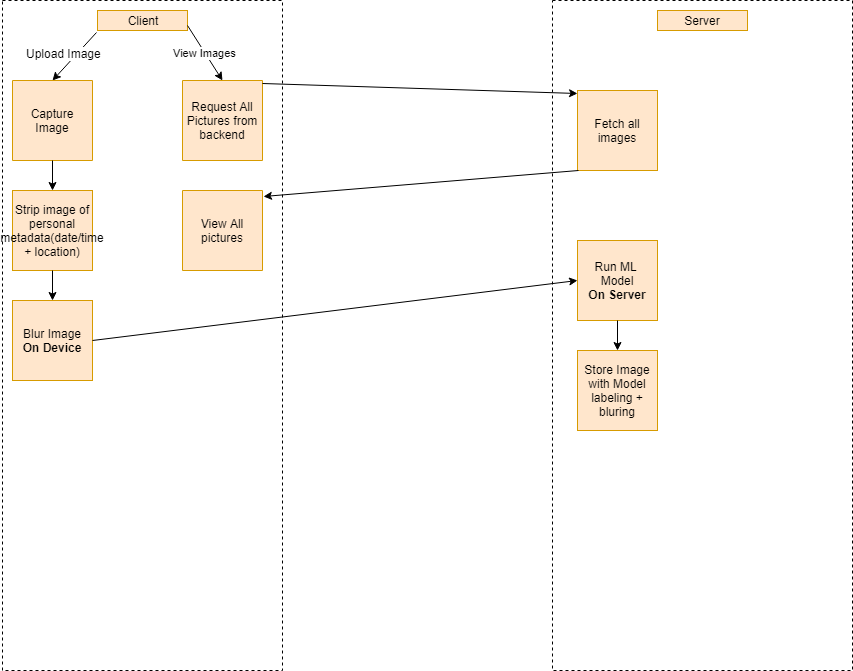
\includegraphics[scale=0.4]{Non}
  \caption{Anonymization Architecture}
  \label{fig:Non}
  \end{figure}
  \begin{figure}[H]
    \centering
    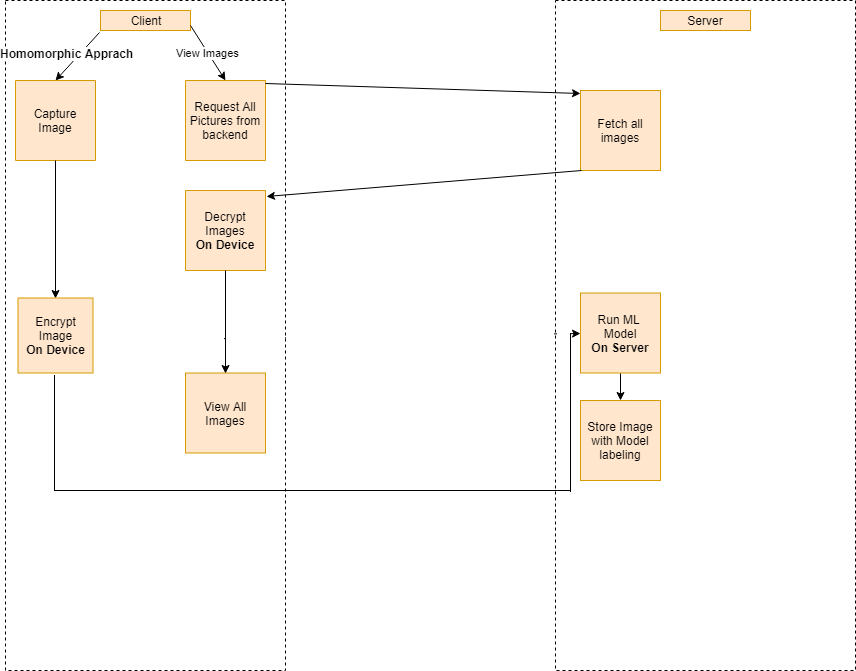
\includegraphics[scale=0.55]{Encrypt}
    \caption{Homomorphic Architecture}
    \label{fig:Encrypted}
    \end{figure}
\subsection{System Design}
The system consisted of a cross-platform Instagram-like mobile application that was developed using Facebook's React-Native, As for the backend we opted for Google's Firebase as the backend provider as it provided multiple advantages over other competitors namely, seamless authentication,
realtime database that was shared across all platforms, access to built-in on device and cloud basic Machine Learning models such as facial recognition and object recognition, the ability to deploy custom Machine Learning (ML) models within the same server and lastly, the ability to scale easily.
The application was developed alongside 2 of my colleagues who were working on similar bachelor projects (personalization and brand recognition).

A social application was chosen to get the most user interaction which in turn would mean more user data to pass of the ML model.
The application flow was as follows, users had  to first sign-up to be able to use the application then, whenever a user signed up the application would prompt the user to verify his email address however this feature was later removed as the majority of the users weren't willing to verify their email-addresses and other wanted to use fake emails as a form of identity security, the user would also get a prompt to choose his Social Interaction Level which changes how his data is handled,
the user would then get a daily notification to post one or more images/text posts while the experiment was running until the thesis submission date.
Users also had the ability to “like” any image posted by any other user to further their preferences. 
\begin{figure}[H]
    \centering
    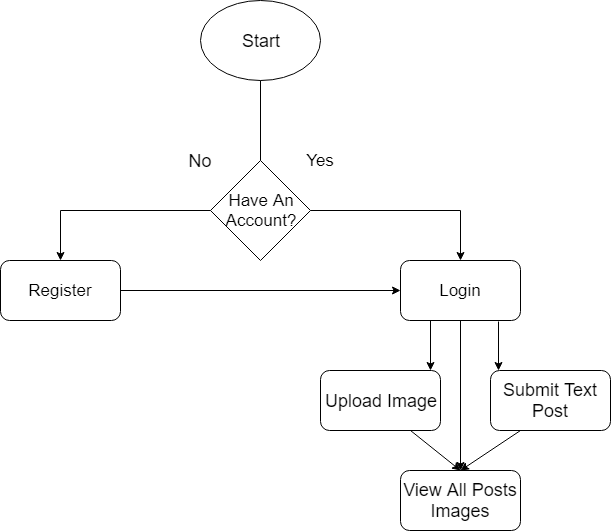
\includegraphics[scale=0.55]{FlowUpdate}
    \caption{In the following figure is the flow of our system}
    \label{fig:flow}
    \end{figure}
We decided to use Google's Material Interface guidelines not only because it simplifies the user interface as much possible but also due the simplicity in implementation it offers. We chose bright colored buttons and cards in addition to being consistent with our design choices such as button placements,validation errors to make the experience more enjoyable and intuitive so we could increase user retention as much as we could.
\begin{figure}[H]
    \centering
    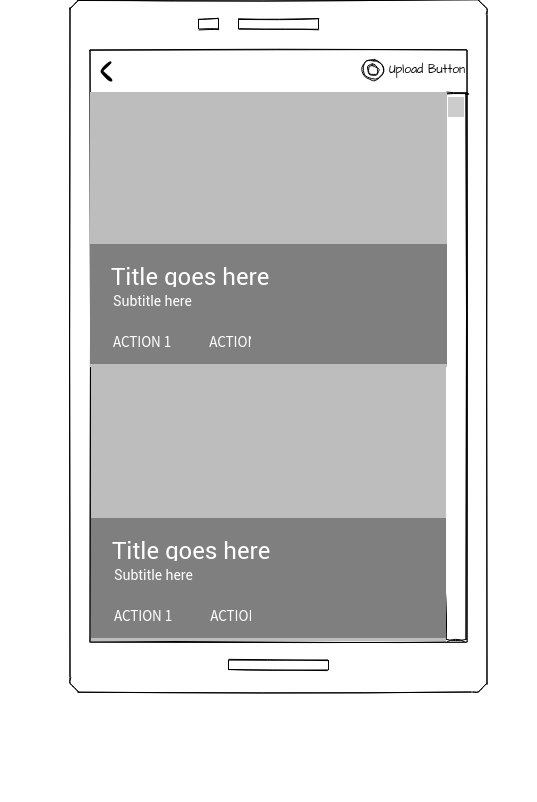
\includegraphics[scale=0.25]{Timeline}
    \caption{In the following figure is a wireframe of the user's timeline }
    \label{fig:Timeline}
\end{figure}
We tried to follow an incremental approach while developing the application where we ranked all the features in order of priority from highest to lowest, we prioritized shipping the most important features first such as the Login/SignUp process and the ability for users to upload images to our database even if it wasn't shown to them in the UI so our data-collection would start as early as possible, followed by features of lessar importance such as improving the user experince and working on multiple security features for the backend and patching bugs.
This was acceptable to the majority of the users since the audience that was targeted understood that the application was an experimental application rather than a production-ready application.
\newline
\newline
At the end of development, the application consisted of 5 different screens being, Login, Register, A Questionnaire, Top Photos and Timeline. The login and registration screens are self-explanatory, as for the questionnaire it was shown upon registration only and was used to put to gather intial preferences about tech items and clothing items the users prefered the most so my colleague would be able to start the personalization process, similary the top photos screen was also shown once following the
registration of any user and the completion of the previously described questionnaire, the top photos screen asked the users to input their most favourite pictures that they would like to share whether it was images of themselves or clothing/tech items they liked.
We also offered users an option to opt-out of reminding notifications while they were registering as some users reported their refusal to allow our application to get the notification permissions on android, however this was in a later build that wasn't ready so most users couldn't benefit from it. 
\newline
\newline
\newline
\newline
\newline
\begin{figure}[!ht]
  \centering
  \begin{minipage}{.55\textwidth}
    \centering
    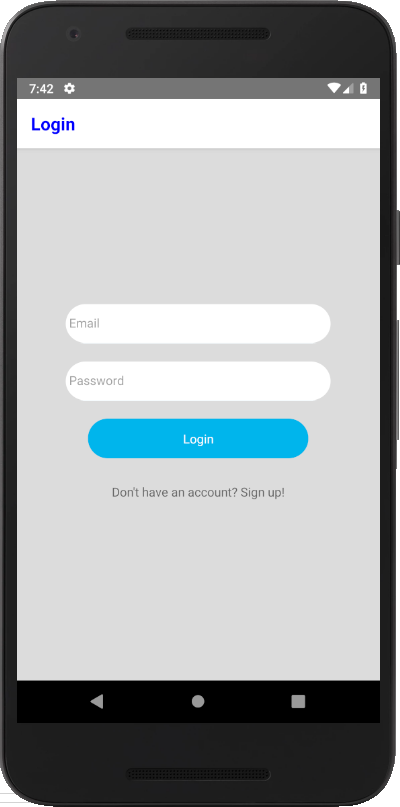
\includegraphics[width=.5\linewidth]{Login}
    \captionof{figure}{Login Screen}
    \label{fig:blur}
  \end{minipage}%
  \begin{minipage}{.55\textwidth}
    \centering
    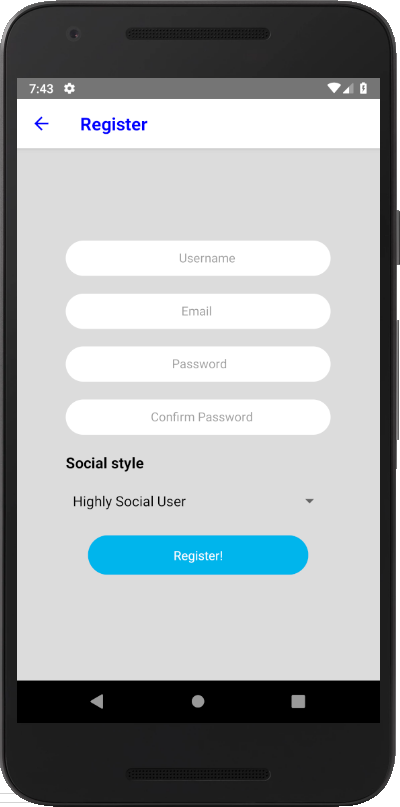
\includegraphics[width=.5\linewidth]{Register}
    \captionof{figure}{Registeration Screen}
    \label{fig:censor}
  \end{minipage}
\end{figure}
\subsection{Homomorphic Scheme}
We had previously outlined three potential libraries to use for Homomorphic Encryption(HELib,SEAL,PALISADE). We decided to use SEAL as it proved the most beneficial to us.
Since the goal was to use Homomorphic Encryption on a mobile platform which was not natively supported by any library as of the time of writing this, We had to re-compile the SEAL library which was written in C++ and compile it using Javascript to be compatible with our React Native application.
There was no direct conversion available to either convert the C++ code into Javascript or compile C++ directly into Javascript, however what we found was that React Native offers what is called Native Modules, Native Modules are basiaclly either native android code (Java) or native iOS code (Swift) that are linked to Javascript using what is called React Native Bridge which exposes native methods to Javascript.
So our goal now to first compile the C++ SEAL library into Java first then link the produced Java library to Javascript using the React Native Bridge.\par

In general, to run C/C++ code using Java it is done through the Java Native Interface (JNI) which acts as a bridge between Java and C/C++ source file. This process was done as follows, First, we had to use the provided CMake file which is used to manage the building process in a compiler independent manner to import the source files into Android Studio and package them into a library, for this process a lot of errors were encountered due to compatibility issues with different versions of CMAKE.
After managing to port the library into Android Studio and connecting it to our React Native application, the next step was to feed the encrypted data to our neural network however this was not possible as all pre-built Machine Learning libraries and APIs don't support this kind of data format as all of the libraries are designed to take the data directly without any change. We then figured out that it was necessary to build our neural network from scratch starting from the filters and kernels to the activation functions meaning we would essentially have to build our own library which proved to be too challenging and time consuming for this bachelor thesis since we had no prior knowledge of Machine Learning
and Neural Networks.


\section{Data Anonymization and Incremental Privacy}
\label{Part:PrivacyLev}
For this part we discuss how multiple Data Obfuscation techniques were used for user submitted data in the application we built instead of using Homomorphic Encryption.
Secondly, what our approach for Incremental Privacy was, how we implemented it and applied it to the 2 closely related synthetic datasets that were generated, One was designed for friendship inference between students in the GUC and the other one was designed for location inferencing between
students in similar tutorial groups in the GUC, which we will be discussing in later sections in full detail, to test how Incremental Privacy would affect our Machine Learning Models.
\subsection{Data Anonymization}
The main idea in this scheme was to allow the user to choose his own level of privacy by having the user choose his desired social interaction and privacy during the registration process which would affect his experience in the application later on. We defined 3 privacy/social levels for the users to choose from. The levels being, Highest Social Interaction, Medium Social Interaction user and lastly a Non-Social User. Each level then would have certain data anonymization techniques applied to his data.
High Social Users had all their data as it as without any modifications to their images and text submitted, On the other hand Medium Interaction users had all their image run on a trained face detection machine learning model and applied blurring over resulting faces. These user’s text posts however were posted as it as without any filtering.
Lastly, the Non-Social users had the most privacy out of the three levels, For images they had the blurring and face detection algorithm run in addition to removing in metadata in images submitted such as location and date.\par

The model used for facial detection is an *on-device* model to ensure privacy and is provided by Google’s firebase ML Kit, as for the blurring, All javascript image manipulation libraries weren't compatible with React Native hence, we were forced
to build our own blurring algorithm using native Java which was pretty straight-forward and consisted of running Google's Firebase ML Kit to detect the faces in the input image then we applied the blurring algorithm on the bounding boxes returned from the face detection model finally, we passed the resulting image back to React Native using React Native Bridge.\par

As for The text posts of these users was also filtered to prevent any locations,names and phone numbers from appearing using a Javascript Natural Language Processing library  “Compromise”\cite{Compromise}. We have also added local GUC landmarks and buildings to the lexicon of the library which detects these words when they are used in any form.
\begin{figure}[!ht]
    \centering
    \begin{minipage}{.5\textwidth}
      \centering
      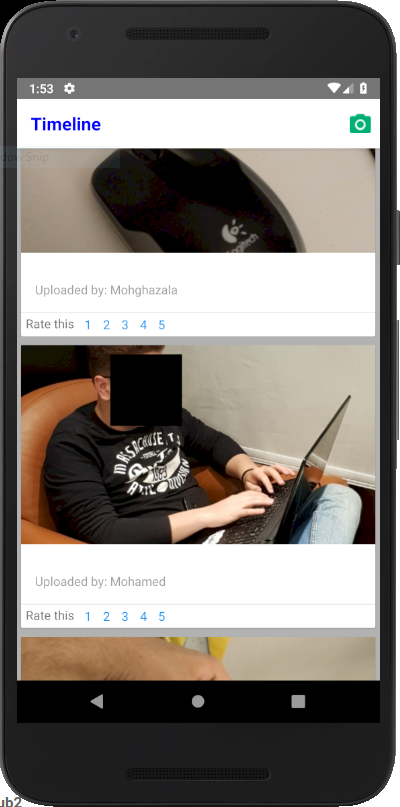
\includegraphics[width=.6\linewidth]{Blur}
      \captionof{figure}{Test User with blurred face}
      \label{fig:blur}
    \end{minipage}%
    \begin{minipage}{.5\textwidth}
      \centering
      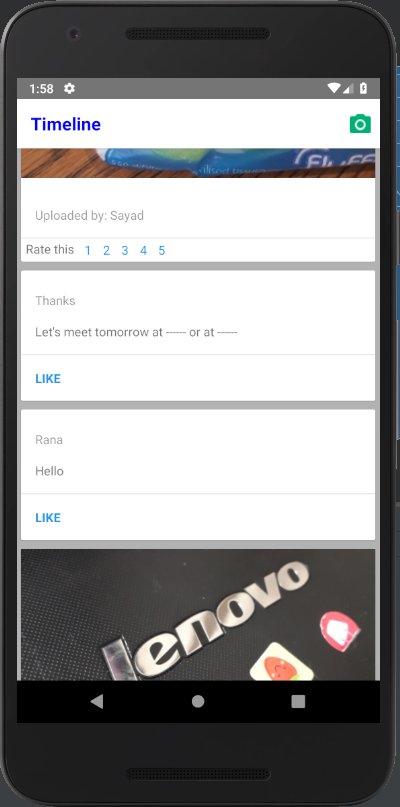
\includegraphics[width=.6\linewidth]{Censor}
      \captionof{figure}{Censored text with location Data}
      \label{fig:censor}
    \end{minipage}
\end{figure}
\subsection{Dataset Generation}
Our initial goal was to test the Data Obfuscation and Incremental Privacy locally on students from the GUC however since there was no publicly available dataset from the university, we had to resort to generating our own synthetic Dataset.
Synthetic Dataset generation is commonly used for research purposes as it can be customised to fit the needs of any particular research topic moreover, Institutions and Organizations
have been hesitant to publish any results using any datasets that have been collected from their customers due the recent growing privacy concerns worldwide\cite{dandekar2018comparative}  espically in the EU after 
the latest General Data Proctetion Regulation (GDPR) laws have been passed.
The generated data varies according to the application and research field and may often include text,social connections,images,graphs. The simplest way to generate such datasets is to create
multiple scripts each handling a specific part of the problem the research is tackling and then combine all related rows of data.\cite{albuquerque2011synthetic}\par

In this paper we chose to use Python to generate our datasets as it has multiple data manipulation libraries namely Numpy and Pandas which are both part of the SciPy package for Python\cite{SciPy}.\par

For the student friendship prediction dataset we tried to make it as realistic as possible to avoid making it too easy to learn. We tried to model the data that could be generated from 1st year students in a 1 month duration, The design was as follows, each student had a name, 5 intrests chosen randomly out of 20 pre-determined intrests,a tutorial group
that the student is assigned to and finally, each student had a number of “events” that represented his online social presence which could resemble tags in pictures,Facebook mentions,Facebook posts.
To make it more realistic each event had a random number of students participating in it, these students were selected in 2 phases, the first phase was used in the 15 days of the modeling process
where students were selected to be in other student's events randomly which resemble the process that students usually go through when they first join an institution where they are introduced to a large amount of
people as they are seeking to make new friends however as time passes each student's social circle is further reduced to people who are considered friends rather than random people met in lectures, we tried to achieve this
in the final 15 days of the 1 month modeling period by making the participants of the remaining events based on the mutual intrests of students and the number of their previous appearances in the first 15 days of the modeling process.
After generating the data for 150 students we then used cross product to get a record for every student with all the others and finally, to decide whether every 2 students should be friends or not, we designed an equation with what we felt
was the most realistic weights for each parameter described above and the final equation was as follows:
\begin{equation}
\small
F=0.15(CommonTutorial)+0.3(MutualIntrests/3)+0.50(MutualEvents/15)^2 +0.5(CommonFavLoc)
\end{equation}
\newline
55\% of the weight was given if the number of shared events between the 2 students during the 1 month period was 15 or more events, 30\% of weight was given if the students had atleast 3 mutual intrests
and the last 15\% were given if the students shared the same tutorial. We also considered the values $F$  $>$ $=$ 0.56 to avoid having un-realistic relations.
We ended up with \num{22052}  rows and we provide a sample table with values taken from the dataset below \ref{tab:Friendship Dataset}
We also added the result of the function to each row of the dataset for verification purposes but it is not shown in the table below due to space limitations.
\newline
\newline
\newline
\newline
\newline
\newline
\begin{singlespace}
  \begin{table}[!h]
    \small
    \addtolength{\tabcolsep}{-4pt}
    \begin{tabular}{|l|l|l|l|l|l|l|}
    \hline
    \multicolumn{1}{|c|}{\textbf{Common\_Tut}}             & \textbf{Common\_Loc}                                  & \multicolumn{1}{r|}{\textbf{Mutual\_Events}}           & \textbf{Mutual\_Intrests}                              & \textbf{Friendship}                                    & \textbf{Id1}                                           & \textbf{Id2}                                           \\ \hline
    \textbf{1}                                             & \textbf{0}                                             & \textbf{3}                                             & \textbf{2}                                             & \textbf{0}                                             & \textbf{0}                                             & \textbf{1}                                             \\ \hline
    \textbf{1}                                             & \textbf{0}                                             & \textbf{2}                                             & \textbf{0}                                             & \textbf{0}                                             & \textbf{0}                                             & \textbf{2}                                             \\ \hline
    \textbf{0}                                             & \textbf{1}                                             & \textbf{8}                                             & \textbf{2}                                             & \textbf{1}                                             & \textbf{0}                                             & \textbf{3}                                             \\ \hline
    \textbf{\begin{tabular}[c]{@{}l@{}}.\\ .\end{tabular}} & \textbf{\begin{tabular}[c]{@{}l@{}}.\\ .\end{tabular}} & \textbf{\begin{tabular}[c]{@{}l@{}}.\\ .\end{tabular}} & \textbf{\begin{tabular}[c]{@{}l@{}}.\\ .\end{tabular}} & \textbf{\begin{tabular}[c]{@{}l@{}}.\\ .\end{tabular}} & \textbf{\begin{tabular}[c]{@{}l@{}}.\\ .\end{tabular}} & \textbf{\begin{tabular}[c]{@{}l@{}}.\\ .\end{tabular}} \\ \hline
    \textbf{1}                                             & \textbf{0}                                             & \textbf{3}                                             & \textbf{2}                                             & \textbf{0}                                             & \textbf{148}                                           & \textbf{147}                                           \\ \hline
    \end{tabular}
    \caption{Friendship Dataset}
    \label{tab:Friendship Dataset}
    \end{table}
\end{singlespace}

As for the second dataset the goal was to explore whether we could provide location prediction for students inside the GUC and on holidays given their list of friends. Generating the second dataset was much easier since we had the data that resulted from the first dataset such as each student's friend list  in addition to each student's tutorial number
which was also present in the first dataset and how would the accuracy be impacted by the incremental obfuscation of their data as a form of data privacy protection. As for the location data we proceeded similar to the first dataset by generating a random classroom from the GUC that was assigned to each tutorial for 30 rooms. We managed to generate \num{4606} rows and a sample of the dataset is provided below
\newline
\begin{table}[!h]
  \begin{tabular}{|l|l|l|l|l|l|l|}
  \hline
  \multicolumn{1}{|c|}{\textbf{TimeSlot}}                    & \textbf{Tutorial}                                      & \multicolumn{1}{r|}{\textbf{Location}}                     & \textbf{Student}                                       & \textbf{fav\_loc}                                      & \textbf{friends}                                       & \textbf{Id}                                            \\ \hline
  \textbf{Sat 1st}                                       & \textbf{1}                                             & \textbf{C7.301}                                        & \textbf{Student0}                                      & \textbf{9}                                             & \textbf{371114}                                        & \textbf{0}                                             \\ \hline
  \textbf{Sat 2nd}                                       & \textbf{1}                                             & \textbf{D4.304}                                        & \textbf{Student0}                                      & \textbf{9}                                             & \textbf{371114}                                        & \textbf{0}                                             \\ \hline
  \textbf{Sat 3rd}                                       & \textbf{1}                                             & \textbf{C5.304}                                        & \textbf{Student0}                                      & \textbf{9}                                             & \textbf{371114}                                        & \textbf{0}                                             \\ \hline
  \textbf{\begin{tabular}[c]{@{}l@{}}.\\ .\end{tabular}} & \textbf{\begin{tabular}[c]{@{}l@{}}.\\ .\end{tabular}} & \textbf{\begin{tabular}[c]{@{}l@{}}.\\ .\end{tabular}} & \textbf{\begin{tabular}[c]{@{}l@{}}.\\ .\end{tabular}} & \textbf{\begin{tabular}[c]{@{}l@{}}.\\ .\end{tabular}} & \textbf{\begin{tabular}[c]{@{}l@{}}.\\ .\end{tabular}} & \textbf{\begin{tabular}[c]{@{}l@{}}.\\ .\end{tabular}} \\ \hline
  \textbf{Holiday}                                       & \textbf{6}                                             & \textbf{Paris}                                         & \textbf{Student142}                                    & \textbf{3}                                             & \textbf{134135}                                        & \textbf{142}                                           \\ \hline
  \end{tabular}
  \caption{Location Prediction Dataset}
  \label{tab:my-table}
  \end{table}

Finally, we extracted 10 rows from the second dataset that weren't used in neither training nor testing to be used for the purpose of showing a live demo during the defense by hosting our models on a simple website and running the prediction on these extraced rows.
